\documentclass[pdftex]{beamer}
\usepackage[british]{babel}
\usepackage{graphicx}
\usepackage{url}
\usepackage[normalem]{ulem}
\usepackage{tikz}

\mode<presentation>
\usetheme{Warsaw}
\useoutertheme{infolines}

\setbeamertemplate{navigation symbols}{}
\usebeamertemplate*{logo}
\logo{
\includegraphics[height=0.85cm]{../images/cmetlogo.png}}

\title[FOSINT-SI 2014]{Exploring UK Crime Networks}
\author[\#fosintsi14]{Giles Oatley and Tom Crick\\\url{tcrick@cardiffmet.ac.uk}}
\institute[@DrTomCrick]{Department of Computing \& Information
  Systems\\Cardiff Metropolitan University, UK\\\url{http://drtomcrick.com}}
\date{18 August 2014}

\begin{document}

% titlepage
\begin{frame}
\titlepage
\end{frame}

% TOC
\section*{Talk Outline} 
\begin{frame} 
\tableofcontents 
\end{frame} 

\section{Introduction}

\section{Crime Analysis Techniques}

\begin{frame}
\frametitle{Crime Analysis Techniques}
\begin{itemize}
\item {\textbf{First Generation}}
\begin{itemize}
\item Anacpapa charts
\item Maps with coloured pins\newline
\end{itemize}
\pause
\item {\textbf{Second Generation}}
\begin{itemize}
\item Pajek
\item IBM i2 COPLINK2, IBM i2 Analyst’s Notebook3, ORA
\item Detica NetReveal\newline
\end{itemize}
\pause
\item {\textbf{Third Generation?}}
\end{itemize}
%\end{alertblock}
\end{frame}

\begin{frame}
\frametitle{Crime Analysis Techniques}
``{\emph{Social network analysis of the sort we could call ‘third-generation’
would focus much more intensely on the content of the contacts, on the
social context, and on the interpretation of such information.}}''
(Klerks, 2011)\newline\newline

...understanding in a qualitative way the {\emph{behaviour, motivations and
choices}} of the individuals concerned and contributing to a better
understanding of vital {\emph{social processes, power and affinity structures}}.



\end{frame}

\section{Crime Networks}

\begin{frame}
\frametitle{Crime Networks}
\begin{itemize}
\item {\emph{Disambiguating networks -- the meaning of links:}}\newline
\begin{enumerate}
\item Burglary\newline
\item Gun Gangs\newline
\item Retail Theft\newline
\end{enumerate}
\end{itemize}
%\end{alertblock}
\end{frame}

\subsection{Burglary}

{ % all template changes are local to this group.
    \setbeamertemplate{navigation symbols}{}
    \begin{frame}[plain]
        \begin{tikzpicture}[remember picture,overlay]
            \node[at=(current page.center)] {
                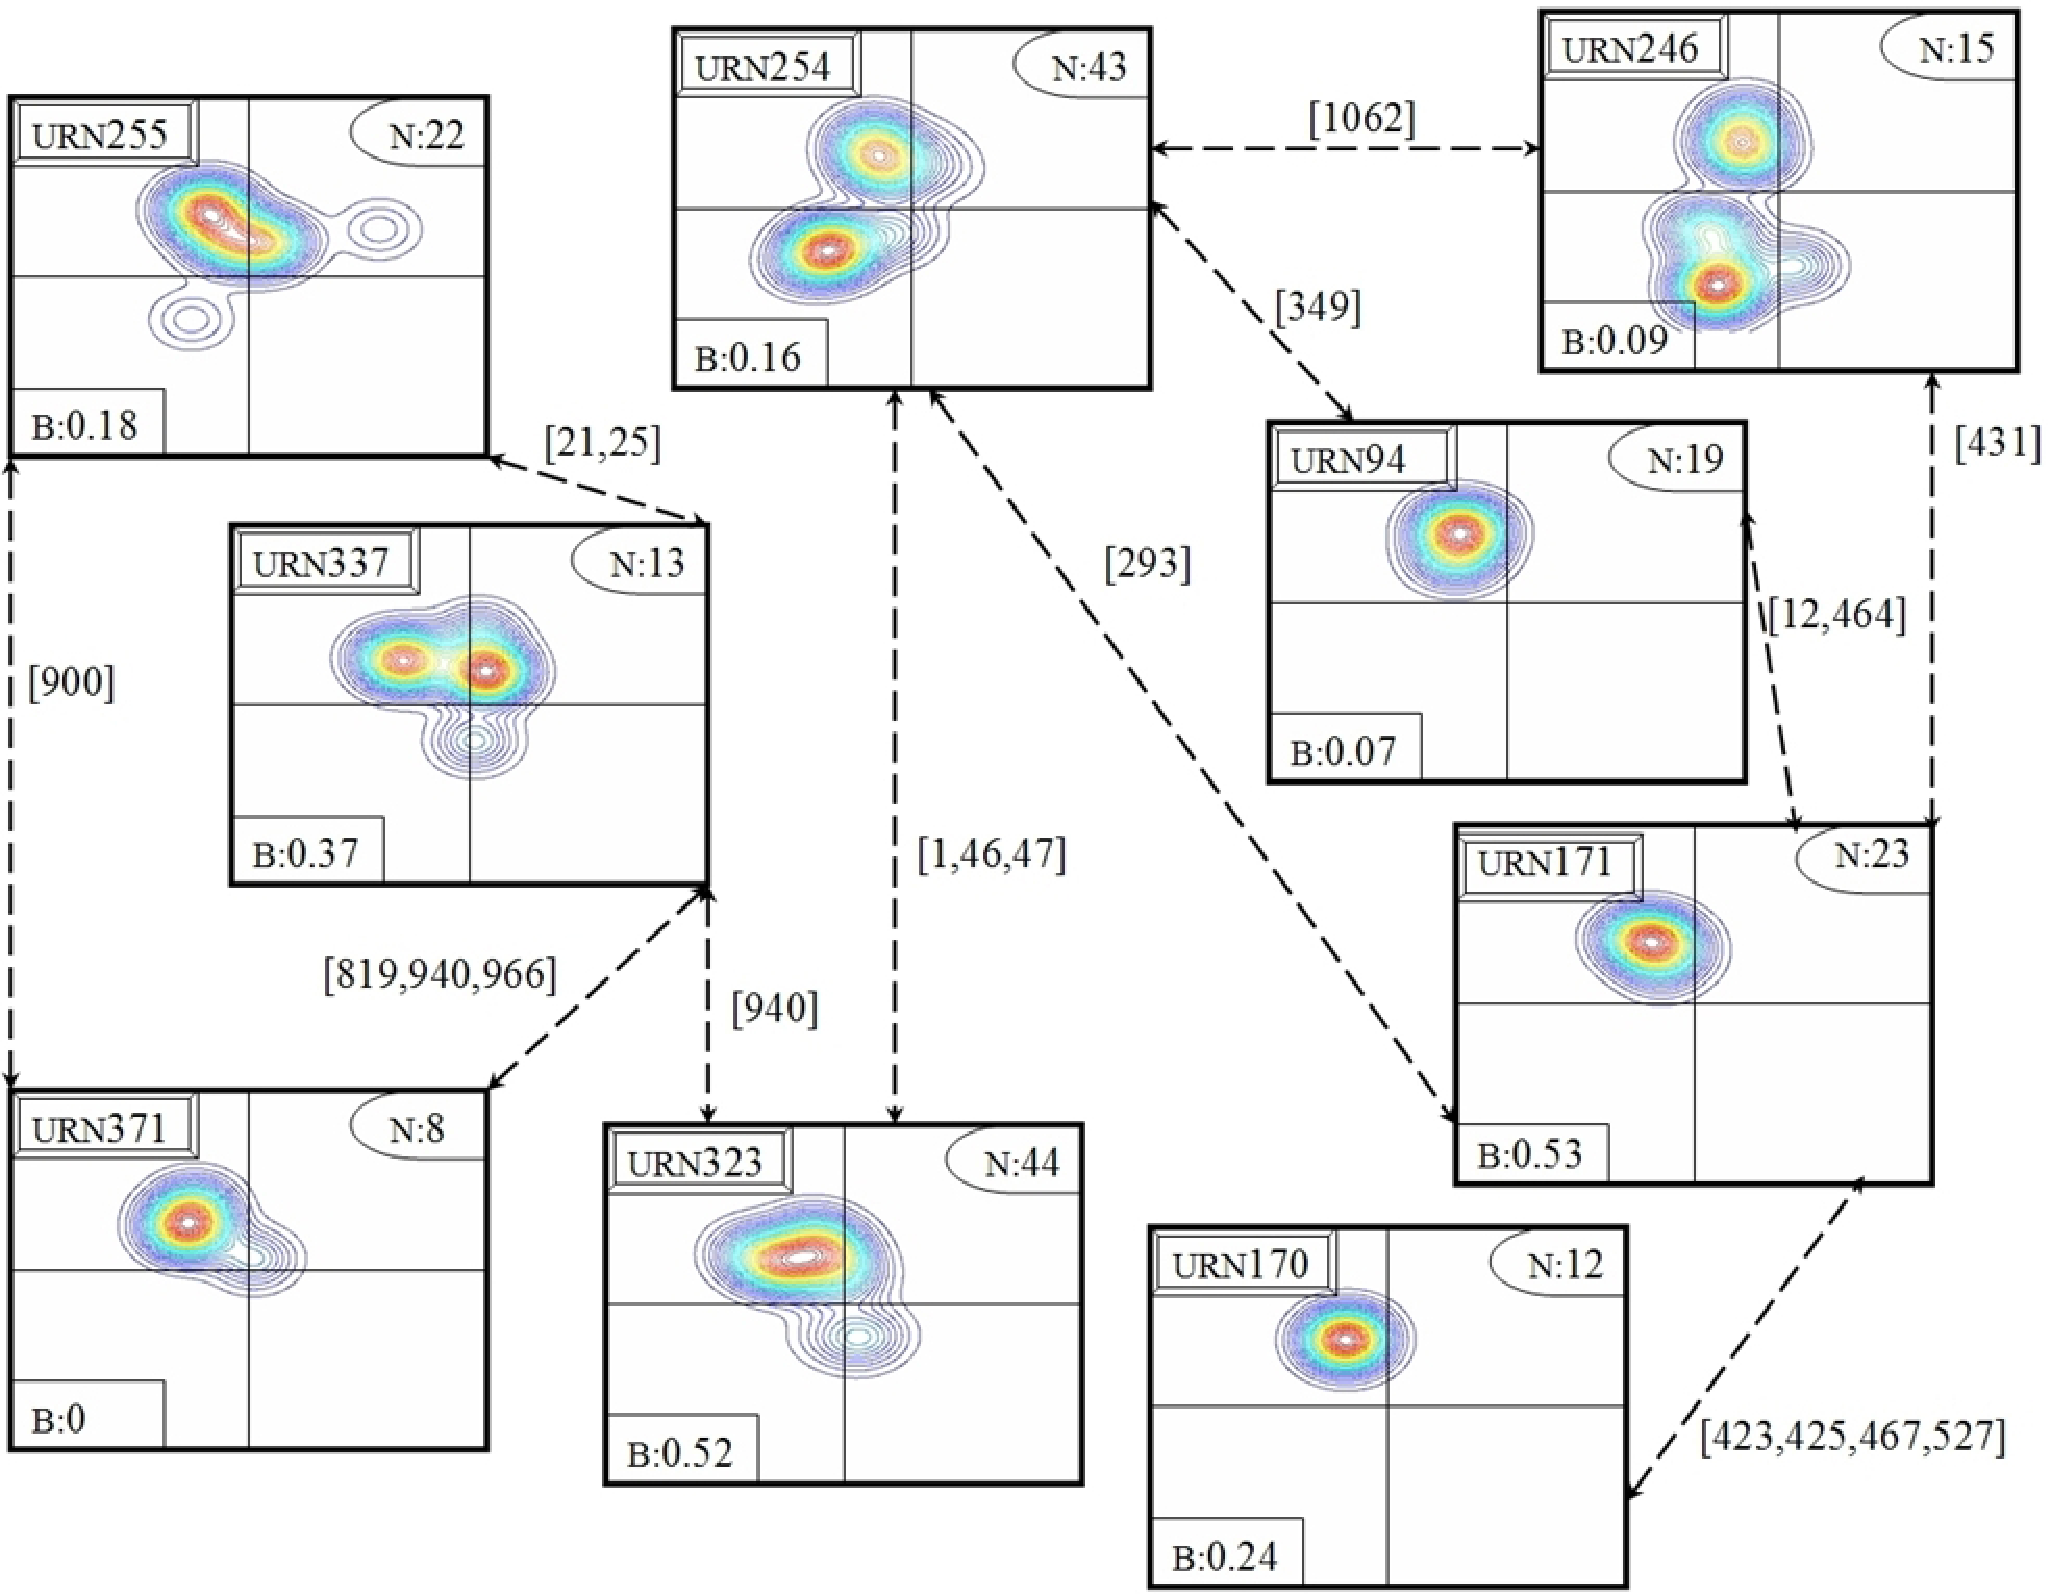
\includegraphics[width=0.9\paperwidth]{../images/burglary.pdf}
            };
        \end{tikzpicture}
     \end{frame}
}

\begin{frame}
\frametitle{Burglary}
\begin{itemize}
\item In conjunction with West Midlands Police, UK
\item Large network of linked offenders ({\emph{n}}=17000)
\item The picture painted by the initial social network plot is
somewhat misleading...
\item The burglary data required spatial data and other features (temporal/frequency) to
  start to understand the meaning of the links between
  offenders
\end{itemize}
%\end{alertblock}
\end{frame}

\subsection{Gun Gangs}

{ % all template changes are local to this group.
    \setbeamertemplate{navigation symbols}{}
    \begin{frame}[plain]
        \begin{tikzpicture}[remember picture,overlay]
            \node[at=(current page.center)] {
                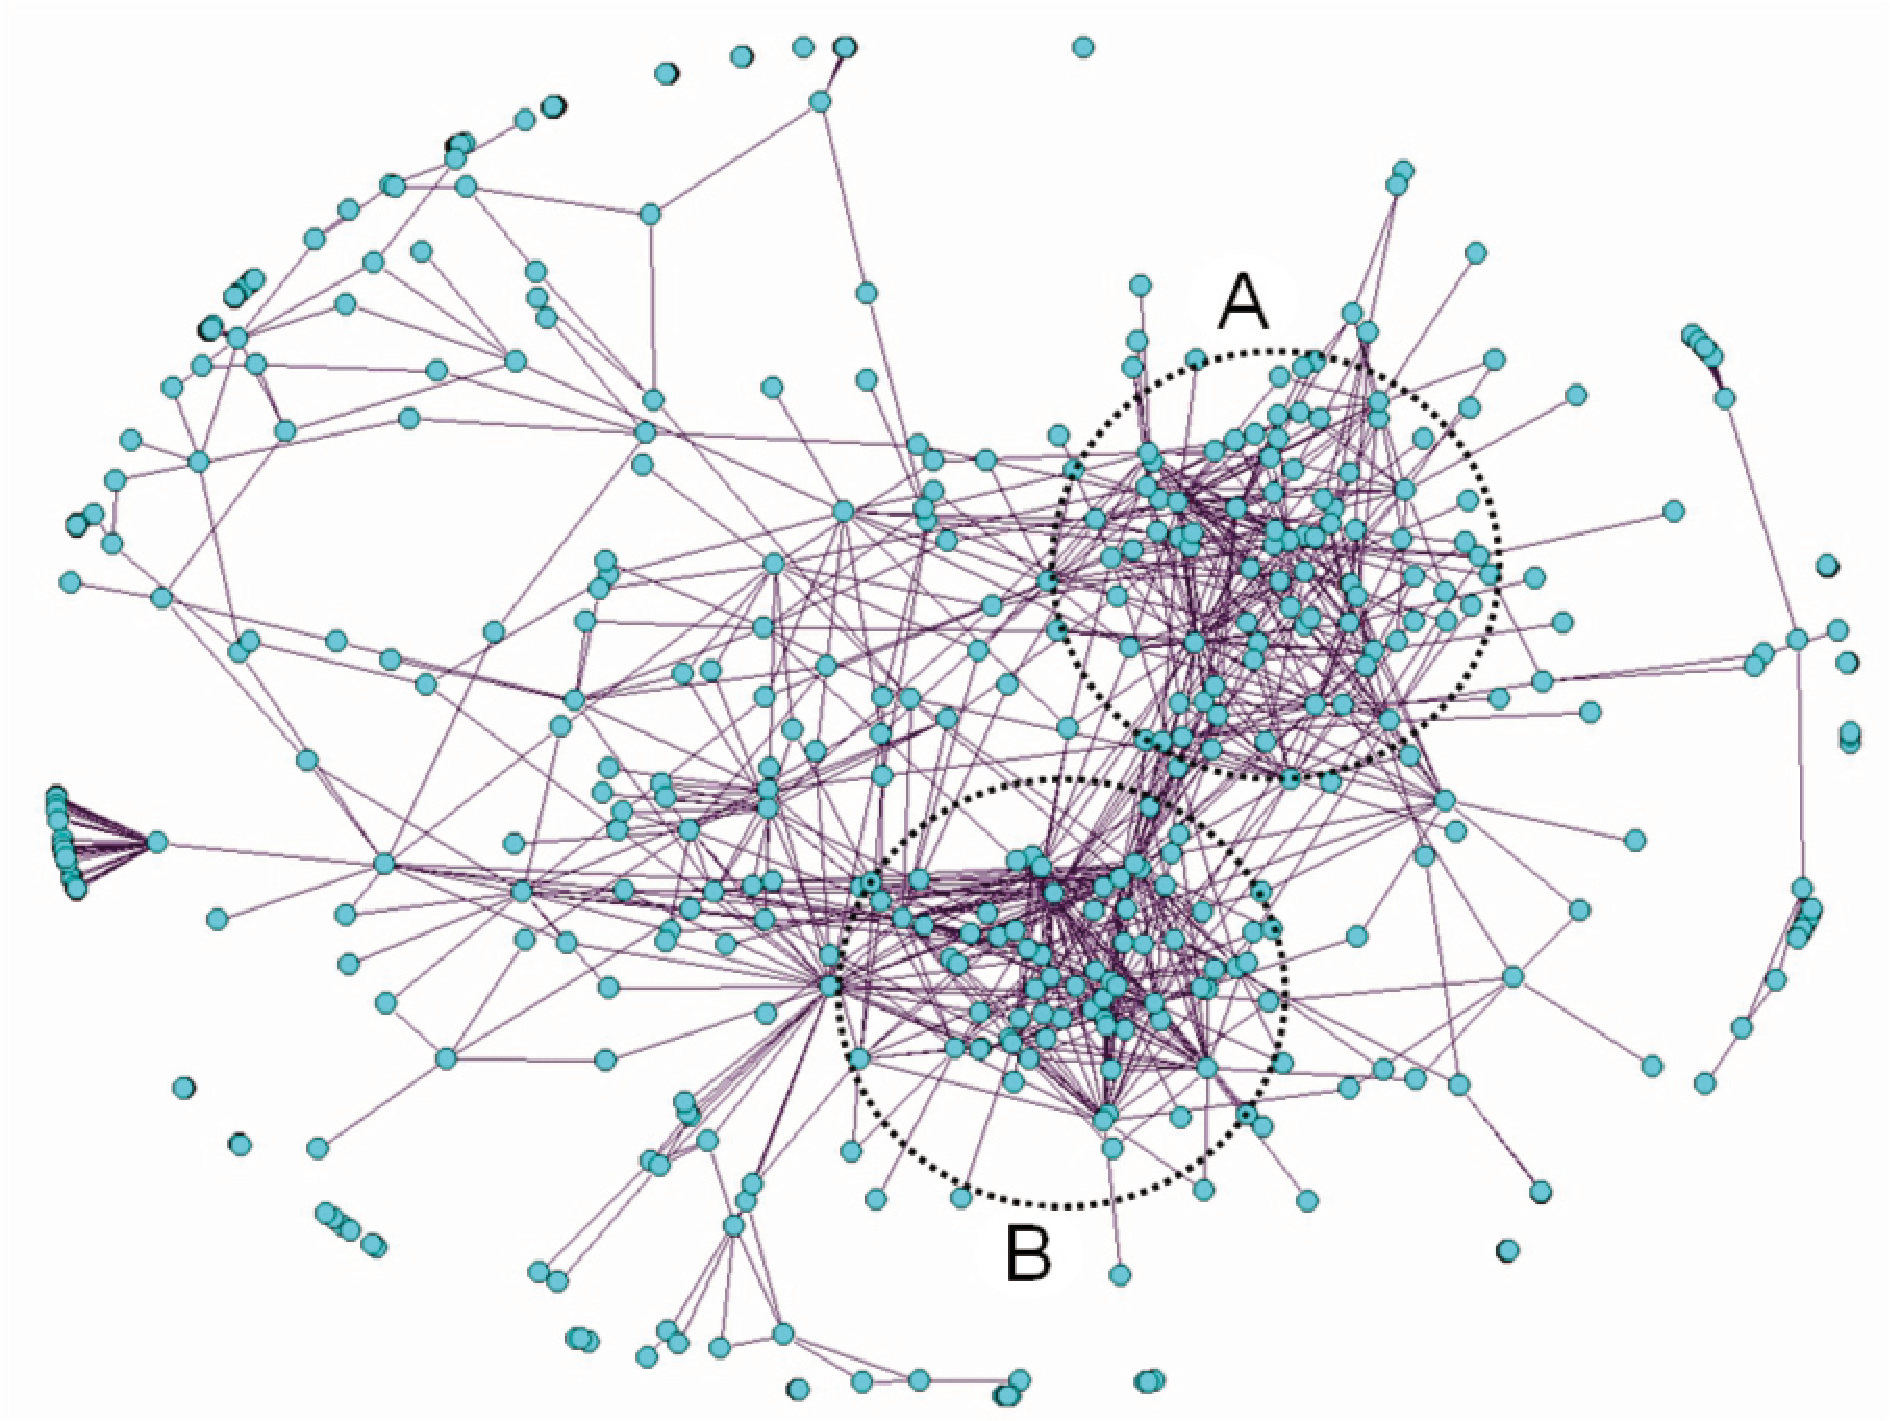
\includegraphics[width=0.9\paperwidth]{../images/2000ganglabels.pdf}
            };
        \end{tikzpicture}
     \end{frame}
}

\begin{frame}
\frametitle{Gun Gangs}
\begin{itemize}
\item In conjunction with Greater Manchester Police, UK
\item Area with a significant gun crime problem, related to gang activity
\item Dynamics of four gangs and their associates
\item Value of SNA for gang research:
\begin{itemize}
\item Identifying structural holes
\item Betweenness
\item Social capital
\end{itemize}
\item Value of third generation analysis
\end{itemize}
%\end{alertblock}
\end{frame}

\begin{frame}
\frametitle{Specific Gang Roles}
\begin{itemize}
\item {\textbf{Leader:}}
\begin{itemize}
\item responsible for recruiting new members
\end{itemize}
\item {\textbf{Provider:}}
\begin{itemize}
\item an individual either internal or external to the gang able to
  supply firearms and/or ammunition
\end{itemize}
\item {\textbf{Enforcers/Riders:}}
\begin{itemize}
\item nominated individuals who are active gunmen for the gang
\end{itemize}
\item {\textbf{Runners/Dealers:}}
\begin{itemize}
\item members of the gang who distribute/supply drugs, usually on the
  leader's behalf; younger members of the group
\end{itemize}
\end{itemize}
%\end{alertblock}
\end{frame}

{ % all template changes are local to this group.
    \setbeamertemplate{navigation symbols}{}
    \begin{frame}[plain]
        \begin{tikzpicture}[remember picture,overlay]
            \node[at=(current page.center)] {
                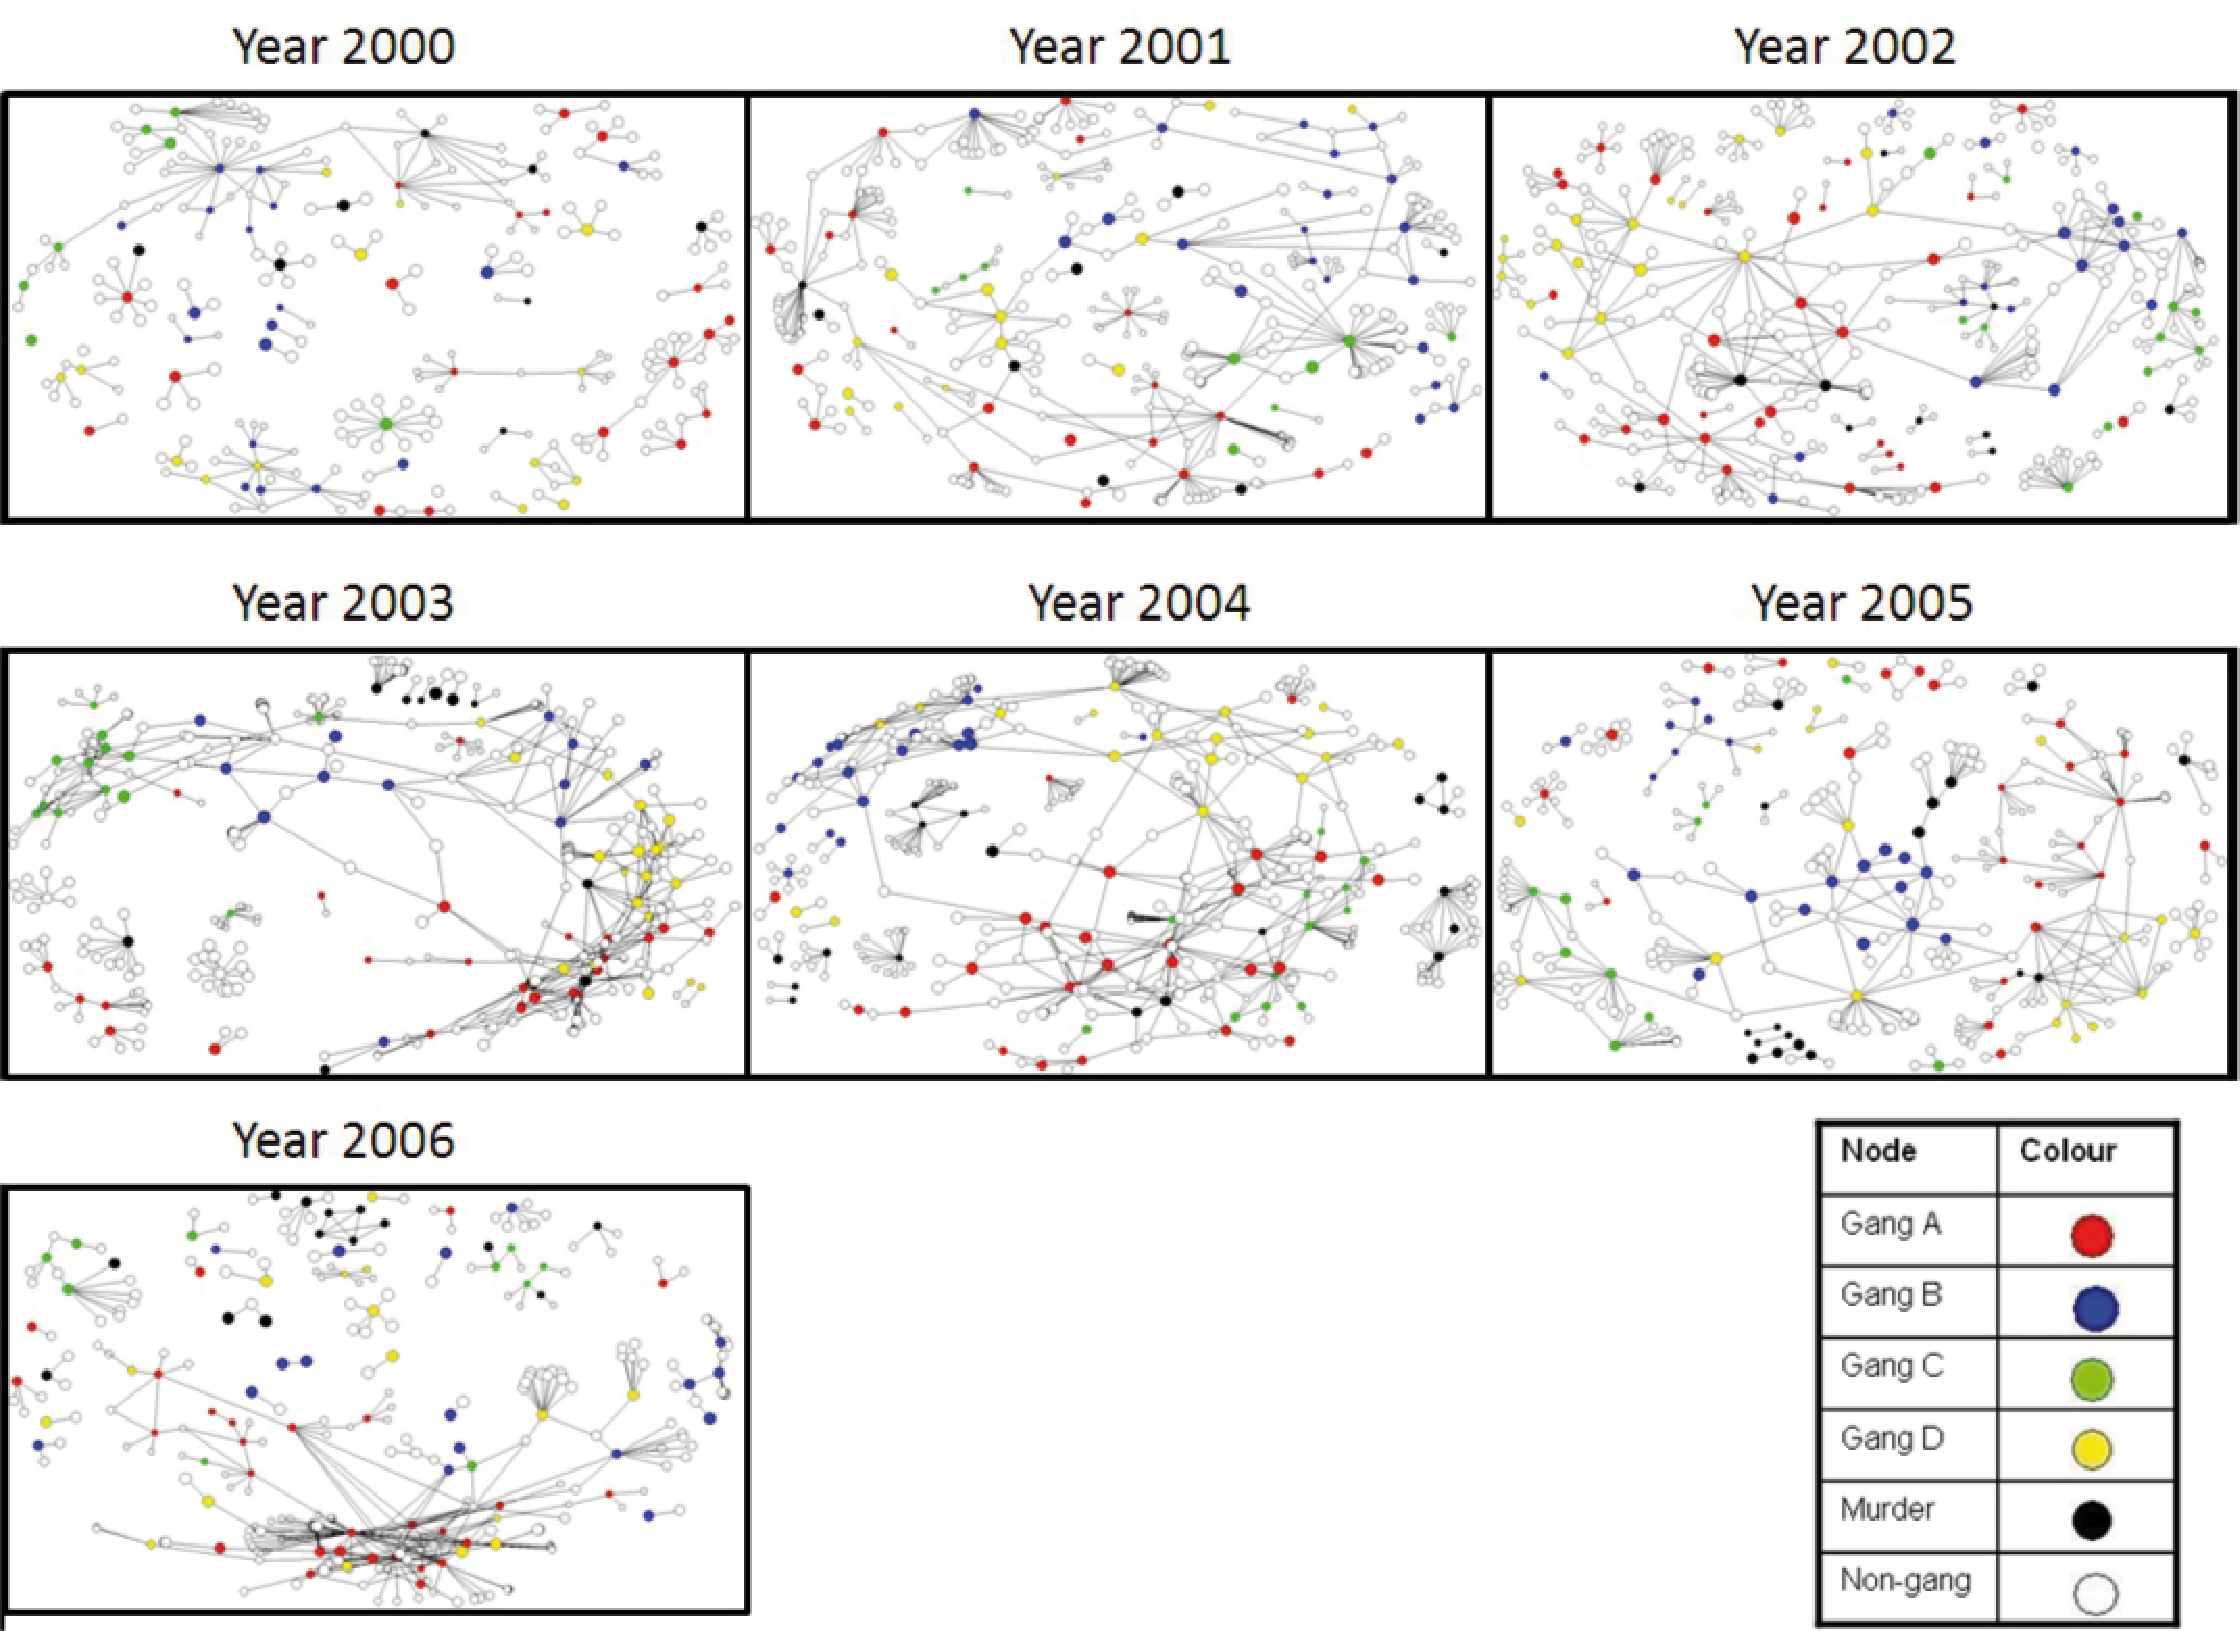
\includegraphics[width=0.9\paperwidth]{../images/all.pdf}
            };
        \end{tikzpicture}
     \end{frame}
}

\begin{frame}
\frametitle{Link Analysis}
\begin{center}
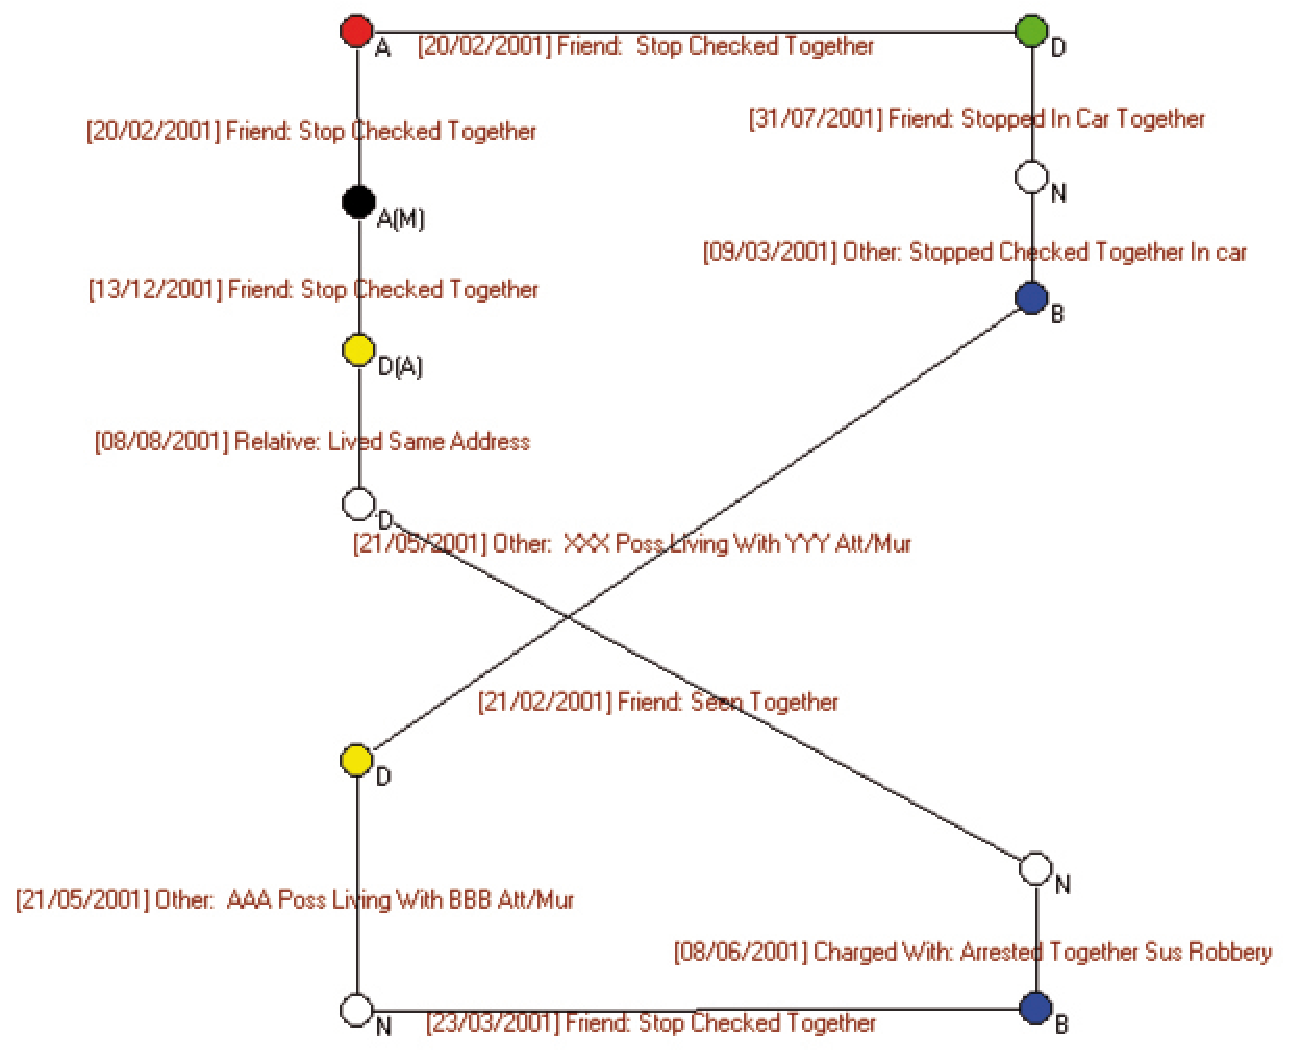
\includegraphics[width=0.48\textwidth]{../images/chain2001.pdf}
\hfill
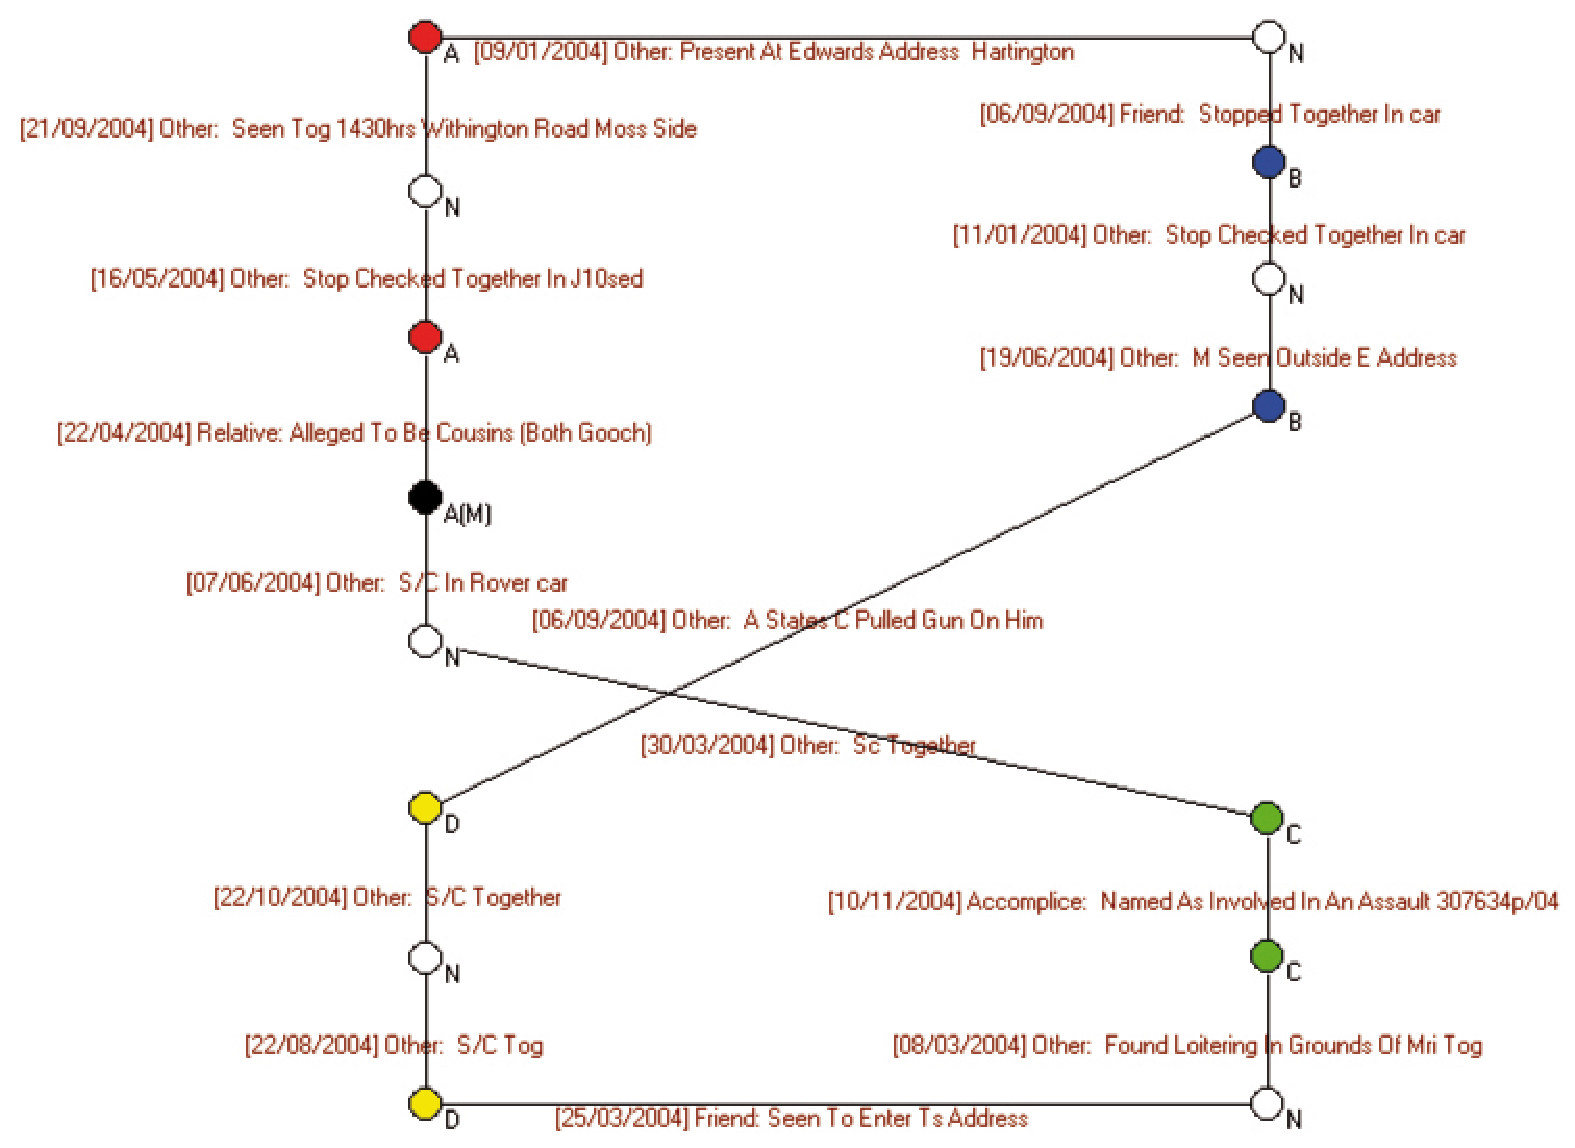
\includegraphics[width=0.48\textwidth]{../images/chain2004.pdf}
\end{center}
\end{frame}

{ % all template changes are local to this group.
    \setbeamertemplate{navigation symbols}{}
    \begin{frame}[plain]
        \begin{tikzpicture}[remember picture,overlay]
            \node[at=(current page.center)] {
                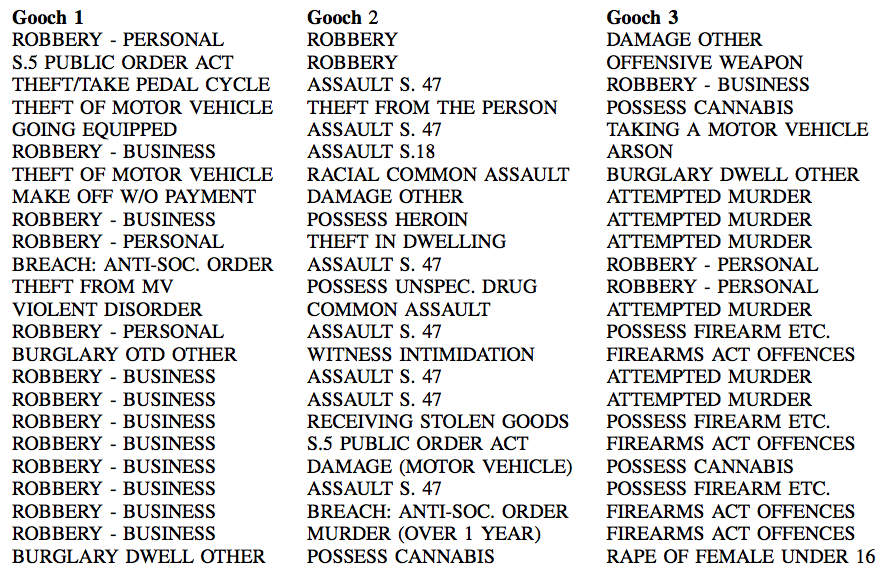
\includegraphics[width=0.9\paperwidth]{../images/offenderhistories.png}
            };
        \end{tikzpicture}
     \end{frame}
}

\begin{frame}
\frametitle{Gun Gangs}
\begin{itemize}
\item The picture painted by the initial social network plot is
somewhat misleading...
\item In the gun gangs, the police-held hypothesis of two rival sets
  of gangs is potentially a misrepresentation of the much more complex
  sets of smaller cliques and fluid changes within the larger gang
  structures.
\item {\textbf{Extremely rich dataset}}; more processing and analysis to follow
\end{itemize}
%\end{alertblock}
\end{frame}

\subsection{Retail Theft}

\begin{frame}
\frametitle{Retail Theft}
\begin{itemize}
\item Unique database from the UK's North East Retail Crime Partnership (NERCP)
\item Partnership between:
\begin{itemize}
\item 29 retail chains
\item 11 shopping centres
\item 6 town/city centre partnerships
\item 4 police forces in the NE of England (+ 11 further forces)
\end{itemize}
\item Information on over 30,000 offenders and 102,000 incidents in
  any 12 month period
\item Complex data of retail crime, with a fraction of known
  gangs, presents its own particular challenges -- how to make use of
  detailed intelligence on individuals (in textual format) and
  combine with mining of the social networks.
\end{itemize}
%\end{alertblock}
\end{frame}

% { % all template changes are local to this group.
%     \setbeamertemplate{navigation symbols}{}
%     \begin{frame}[plain]
%         \begin{tikzpicture}[remember picture,overlay]
%             \node[at=(current page.center)] {
%                 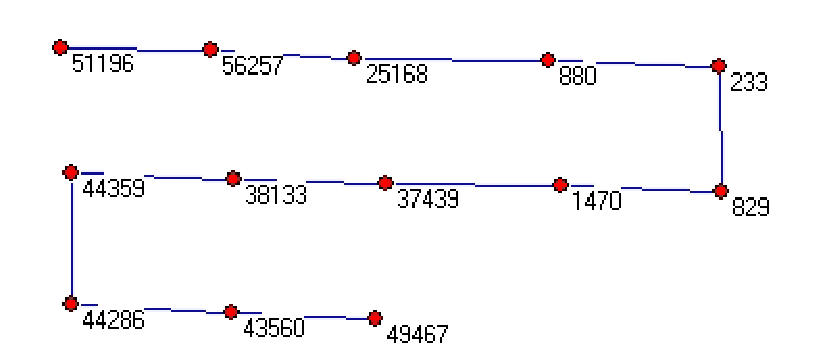
\includegraphics[width=0.9\paperwidth]{../images/path1.pdf}
%             };
%         \end{tikzpicture}
%      \end{frame}
% }

% { % all template changes are local to this group.
%     \setbeamertemplate{navigation symbols}{}
%     \begin{frame}[plain]
%         \begin{tikzpicture}[remember picture,overlay]
%             \node[at=(current page.center)] {
%                 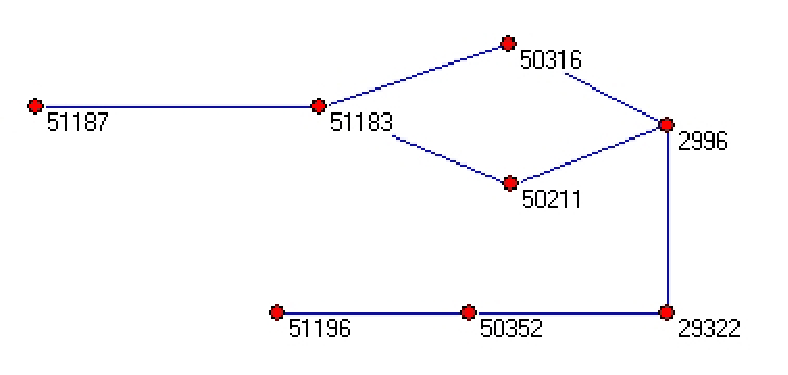
\includegraphics[width=0.9\paperwidth]{../images/path2.pdf}
%             };
%         \end{tikzpicture}
%      \end{frame}
% }

{ % all template changes are local to this group.
    \setbeamertemplate{navigation symbols}{}
    \begin{frame}[plain]
        \begin{tikzpicture}[remember picture,overlay]
            \node[at=(current page.center)] {
                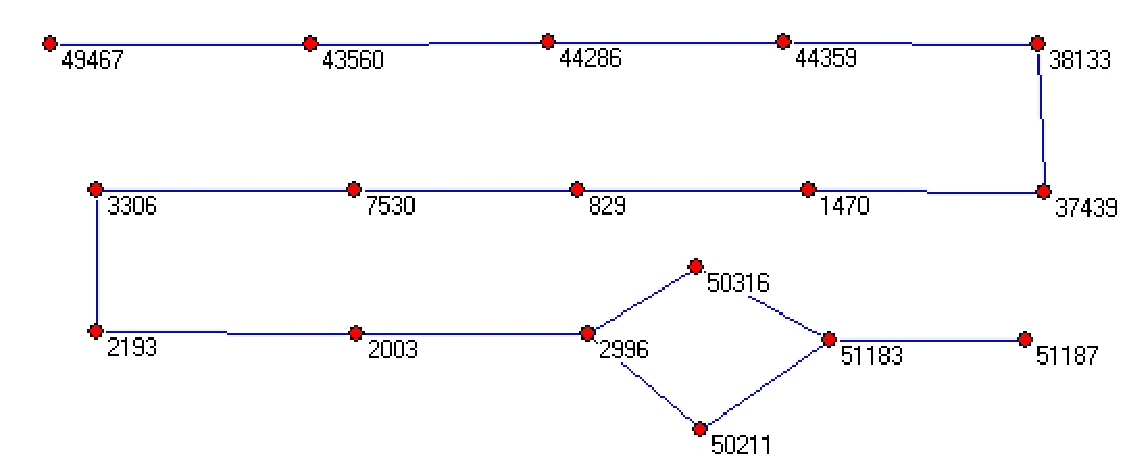
\includegraphics[width=0.9\paperwidth]{../images/path3.pdf}
            };
        \end{tikzpicture}
     \end{frame}
}


\section{Conclusions and Future Work}

\begin{frame}
\frametitle{Conclusions and Future Work}
%\begin{exampleblock}{Some Reasons}
\begin{itemize}
\item The picture painted by the initial social network plot is quite
  misleading in all three cases we have presented:
\begin{itemize}
\item {\textbf{Burglary:}} requires spatial data
\item {\textbf{Gun Gangs:}} pre-existing police understanding of the gangs, not
  complex enough
\item {\textbf{Retail Theft:}} complex, fraction of known gangs, individual intelligence
\end{itemize}
\item How to represent the changing nature of an individual is
  something we have looked at elsewhere, and will continue to do so
\item Also see: {\emph{Measuring UK Crime Gangs}} (ASONAM 2014, S9)
\end{itemize}
%\end{alertblock}
\end{frame}

\begin{frame}
\frametitle{Acknowledgements}
%\begin{exampleblock}{Some Reasons}
\begin{itemize}
\item Acknowledge contributions from:
\begin{itemize}
\item West Midlands Police, UK
\item Greater Manchester Police, UK
\item North East Retail Crime Partnership (NERCP)\newline
\end{itemize}
\item Papers and presentations:
  \url{https://github.com/tomcrick/FOSINT-SI2014}\\
\url{https://github.com/tomcrick/ASONAM2014}\newline
\item Contact: \url{http://drtomcrick.com}

\end{itemize}
%\end{alertblock}
\end{frame}


% { % all template changes are local to this group.
%     \setbeamertemplate{navigation symbols}{}
%     \begin{frame}[plain]
%         \begin{tikzpicture}[remember picture,overlay]
%             \node[at=(current page.center)] {
%                 \includegraphics[width=\paperwidth]{brain.pdf}
%             };
%         \end{tikzpicture}
%      \end{frame}
% }

\end{document}
